
\section{Resultados}

\subsection{Red de interacciones inicial}


\begin{figure}[h] % [h] indica que queremos la imagen aquí, en la posición actual
	\centering
	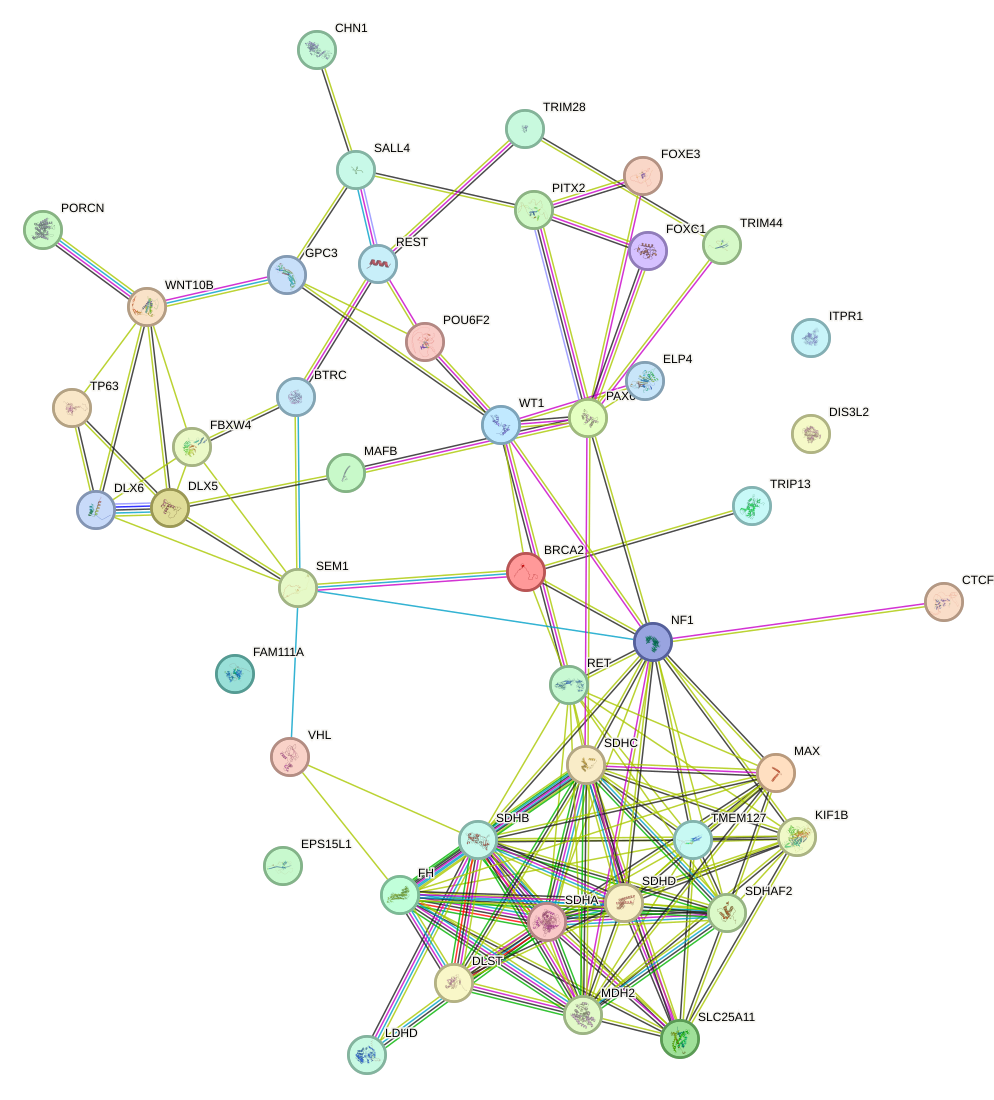
\includegraphics[width=1\textwidth]{figures/red_interaccion_aniridia.png} % Especifica la ruta y el tamaño
	\caption{Red de interacción con los genes asociados al fenotipo HP:0000526} % Agrega una leyenda si deseas
	\label{fig:mi-imagen} % Etiqueta para referenciar la imagen en el texto
\end{figure}

\subsection{Clustering}

\begin{figure}[h] % [h] indica que queremos la imagen aquí, en la posición actual
	\centering
	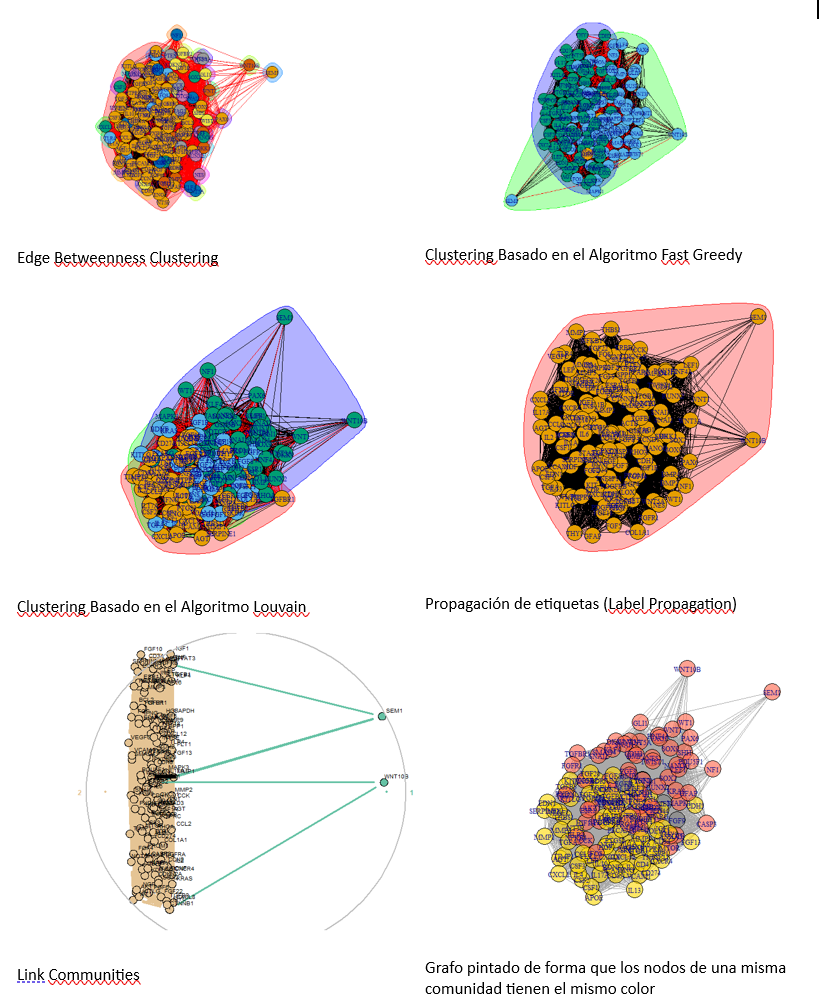
\includegraphics[width=1\textwidth]{figures/toda_figuras_clustering.png}
	\caption{Figuras obtenidas al aplicar clustering con distintos métodos}
	\label{clustering}
\end{figure}

Principalmente el estudio de los resultados se centrará en los genes semilla (WNT10B, WT1, SEM1, PAX6, NF1). En común, se puede observar que SEM1 aparece en varisa posiciones destacadas en los grafos; WT1 y PAX6 están en regiones densas (centrales) de las comunidades, lo que infica que tienen muchas conexiones internas; y NF1 se sitúa en los bordes de las comunidades, por lo que podría actuar como puente entre diferentes comunidades; y WNT10B también es central en algunas comunidades.